%!TEX root = ../master.tex

\section{Appliance company attacking the consumer}
A manufacturer of appliances can have similar objectives as the \cref{3rdpartyattacktree}.
The attack tree is also very similar as seen on \cref{applianceCompanyTree} and thus the description will not be repeated.
The difference is how the data is obtained.
The third party app develop has direct access to the data and the potential of sending the data through the platform that the application is installed on.
An appliance company needs to obtain the data through the firmware on the appliance and send it through either a network connection on the appliance or through the smart meter.
Although possible these means are less likely than those described in \cref{3rdpartyattacktree}

\afterpage{% Insert after the current page
\clearpage
\KOMAoptions{paper=A3,paper=landscape}
\recalctypearea

\begin{figure}
  \begin{center}
    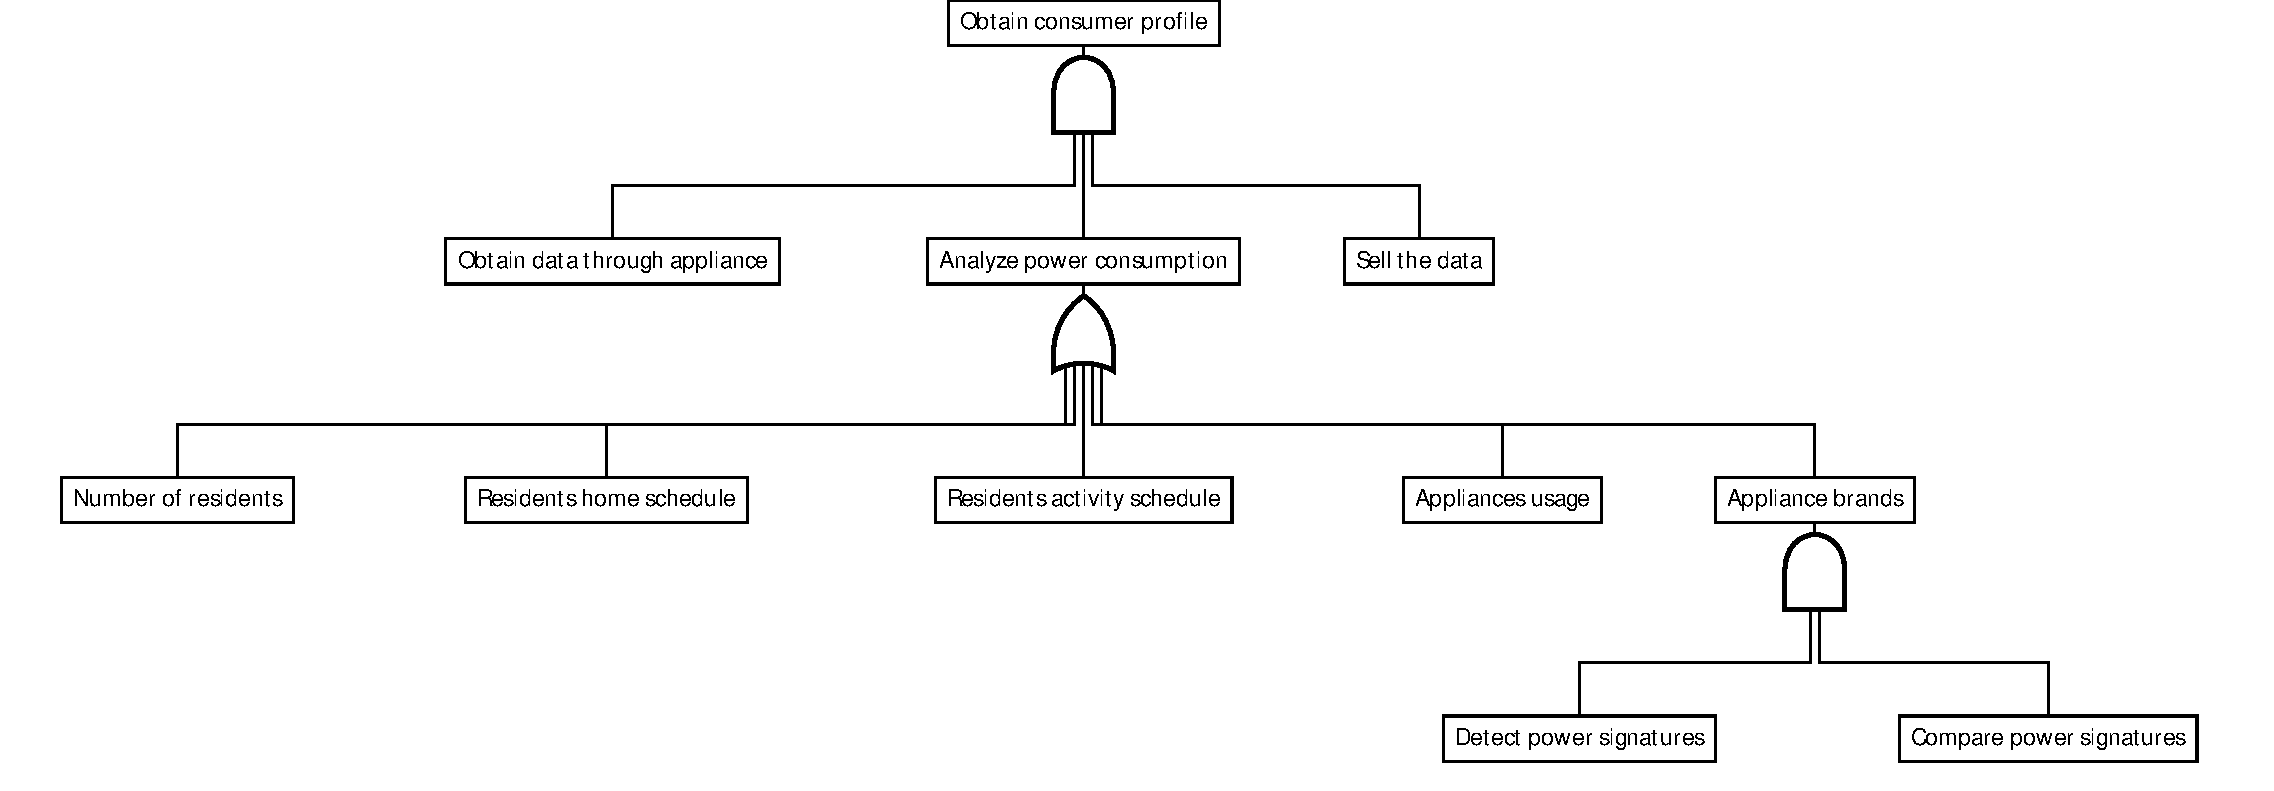
\includegraphics[width=\textwidth]{graphviz/appliancecompany_vs_consumer.pdf}
  \end{center}
  \caption{An appliance company attacking the consumer through their appliance.}
  \label{applianceCompanyTree}
\end{figure}

\clearpage
\KOMAoptions{paper=A4,pagesize}
\recalctypearea
}

